% File tacl2018v2.tex
% Sep 20, 2018

% The English content of this file was modified from various *ACL instructions
% by Lillian Lee and Kristina Toutanova
%
% LaTeXery is mostly all adapted from acl2018.sty.

\documentclass[11pt,a4paper]{article}
\usepackage{times,latexsym}
\usepackage{url}
\usepackage[T1]{fontenc}
\usepackage[utf8]{inputenc}
\usepackage{graphicx}
\usepackage{float}

%% Package options:
%% Short version: "hyperref" and "submission" are the defaults.
%% More verbose version:
%% Most compact command to produce a submission version with hyperref enabled
%%    \usepackage[]{tacl2018v2}
%% Most compact command to produce a "camera-ready" version
%%    \usepackage[acceptedWithA]{tacl2018v2}
%% Most compact command to produce a double-spaced copy-editor's version
%%    \usepackage[acceptedWithA,copyedit]{tacl2018v2}
%
%% If you need to disable hyperref in any of the above settings (see Section
%% "LaTeX files") in the TACL instructions), add ",nohyperref" in the square
%% brackets. (The comma is a delimiter in case there are multiple options specified.)

\usepackage[acceptedWithA]{resources/tacl2018v2}




%%%% Material in this block is specific to generating TACL instructions
\usepackage{xspace,mfirstuc,tabulary}
\newcommand{\dateOfLastUpdate}{Sept. 20, 2018}
\newcommand{\styleFileVersion}{tacl2018v2}

\newcommand{\ex}[1]{{\sf #1}}

\newif\iftaclinstructions
\taclinstructionsfalse % AUTHORS: do NOT set this to true
\iftaclinstructions
\renewcommand{\confidential}{}
\renewcommand{\anonsubtext}{(No author info supplied here, for consistency with
TACL-submission anonymization requirements)}
\newcommand{\instr}
\fi

%
\iftaclpubformat % this "if" is set by the choice of options
\newcommand{\taclpaper}{final version\xspace}
\newcommand{\taclpapers}{final versions\xspace}
\newcommand{\Taclpaper}{Final version\xspace}
\newcommand{\Taclpapers}{Final versions\xspace}
\newcommand{\TaclPapers}{Final Versions\xspace}
\else
\newcommand{\taclpaper}{submission\xspace}
\newcommand{\taclpapers}{{\taclpaper}s\xspace}
\newcommand{\Taclpaper}{Submission\xspace}
\newcommand{\Taclpapers}{{\Taclpaper}s\xspace}
\newcommand{\TaclPapers}{Submissions\xspace}
\fi

%%%% End TACL-instructions-specific macro block
%%%%

\title{Aspect-based sentiment analysis}

% Author information does not appear in the pdf unless the "acceptedWithA" option is given
% See tacl2018v2.sty for other ways to format author information
\author{
  Jaklič, Žan \\ \texttt{63130073} \\ {\tiny \texttt{zj8850@student-uni.lj.si}}
  \And
  Ramovš, Iztok \\ \texttt{63130204} \\ {\tiny \texttt{ir8617@student-uni.lj.si}}
  \And
  Mav, Matjaž \\ \texttt{63130148} \\ {\tiny \texttt{mm3058@student-uni.lj.si}}
}


\date{}

\begin{document}
\maketitle

\iftaclpubformat
\section{Introduction}

A lot of sentiment analysis has been done on short texts, e.g. on tweets, yelp reviews, amazon reviews, and some of the research has been done on longer texts like news, blog posts, etc. There is a lot of incentive to use sentiment analysis on those cases. Such techniques can for example help companies and researchers with understanding of user opinions or filter out unimportant ones. One example for sentiment analysis application can even be predicting how markets will shift due to financial news.

On one side there is interest to assign sentiment to the whole document and on the other, there is interest to assign sentiment to each entity mentioned in the document separately. We will focus on the more scarcely researched second option, called aspect based sentiment analysis, processing a dataset constructed of Slovene news article. 

\section{Related work}

We reviewed the proposed literature and some additional papers, which research the problem of aspect-based sentiment analysis. Across all papers, the majority of recently popular approaches for natural language processing were used. 

First, we read a paper \cite{asghar}, which mostly focuses on data preprocessing and feature extraction. This paper along with most of the others we read recommends heavy preprocessing of the initial texts, including punctuation and stop word removal, transforming letters to lower-case, part of speech tagging and lemmatization. However \cite{c_sentinews}, which analyzes Slovene documents, recommends that we omit stop word and capitalization removal.

Most of the approaches take advantage of machine learning models, while \cite{sweeney} also tried predicting sentiment with lexicons. \cite{biyani} divided the classification problem into several binary classifications, where \cite{ding} used multi-class classification approach. Machine learning models used for classification ranged from Naïve Bayes \cite{c_sentinews}, Support Vector Machines \cite{tang}, to neural networks \cite{jebbara} and transformers \cite{yang}.
There were also a few novel approaches. \cite{jebbara} created custom sentiment embeddings, \cite{wallaart} took the ontology approach, where they transformed words into aspects and classified sentiment based on domain specific rules. \cite{guha} used a special form of clustering instead of word embeddings. \cite{hercig} approached the problem with unsupervised methods. Intel's NLP architect, which is based on \cite{mamou}, uses semi-supervised learning, where a domain specific opinion lexicon is automatically created and can be then manually corrected if needed.

Besides \cite{c_sentinews} we also reviewed another lexicon approach on Slovene texts \cite{kadunc}. We have not had the time to go through the doctoral dissertation \cite{bucar_phd}, but we intend to use it for further guidance in our research project.


\section{Data description}

The corpus we will use is the SentiCoref 1.0 \cite{c_senticoref} which consists of 837 documents and 433 thousand tokens which were selected from SentiNews 1.0 corpus \cite{c_sentinews}. The text contents of those selected documents are from five different Slovene news portals. The SentiCoref corpus is already annotated with following data for each token:

\begin{itemize}
    \item location of token in text,
    \item type of named entities (person, organization or location),
    \item coreference to named entities,
    \item discrete sentiment range from very negative to very positive for each entity. 
\end{itemize}

Most of the annotated sentiment in database is tagged as neutral; the distribution for entities is following: 30 Very negative, 1801 Negative, 10869 Neutral, 1705 Positive and 24 Very positive.

\begin{figure}[H]
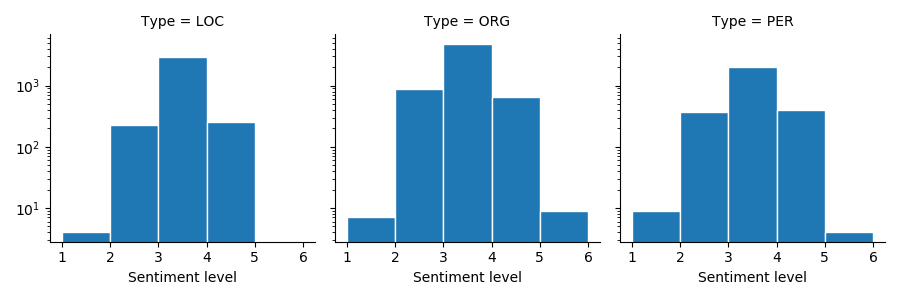
\includegraphics[width=0.5\textwidth]{resources/sentiment_distributions.png}
\centering
\label{fig:sentiment-distribution}
\caption{Sentiment distribution compared to the entity type. Note that frequencies are in logarithmic scale.}
\end{figure}

\section{Project idea}
At the moment we have limited knowledge regarding machine learning models used for advanced language processing. We have therefore decided that we will come to the best options regarding preprocessing, feature extraction, modelling and evaluation through experimental testing. We intend to implement most of the perspective methods studied in related works and will try to develop a few of our own solutions in each of the steps mentioned above.

Our goal is to first build a simple model, so we get familiar with the data and algorithms used, and then improve every process in the pipeline to achieve best results possible.

We will initially use less preprocessed text, as that appeared to yield better results in Slovene texts. We aim to extract the local context of an entity with taking into account a fixed amount of tokens in its neighborhood. Bigrams and word embeddings appeared to be useful for evaluating sentiment in previous research, so we will use them as well. We will use Slovene lexicons to establish a benchmark, and compare them to simpler models, such as Naive Bayes, first. Most of the previous papers used accuracy and F-score for evaluating their results. However we are concerned about the distribution of our sentiment classes, where very polar classes represent a very small number of all cases. 

We aim to improve our results throughout development, with experiments, as we gain more knowledge about our dataset and language processing procedures.

\subsection{Preprocessing}
\begin{itemize}
  \item Parsing initial data
  \item Tokenization
  \item Punctuation and capitalization processing
  \item Part of speech tagging
  \item Lemmatization
  \item Stop word removal
\end{itemize}

\subsection{Data inspection}
\begin{itemize}
  \item Average sentence and word length
  \item Class distribution among entities
  \item Source and domain bias
\end{itemize}

\subsection{Feature extraction}
\begin{itemize}
  \item Local context
  \item Negation, conjuction, superlative evaluation
  \item Punctuation
  \item Ontology based approach
  \item N-grams
  \item TF-IDF, word embeddings
  \item Additional data to expand feature space
\end{itemize}

\subsection{Modelling and evaluation}
\begin{itemize}
  \item Lexicons
  \item Simpler machine learning models
  \item Deep learning models
  \item Transformer models
  \item Stacking
  \item Accuracy, F-score
\end{itemize}

\subsection{Main question for future work}
\begin{itemize}
  \item What is the proper amount of text preprocessing?
  \item How should we evaluate local context of an entity?
  \item Is our dataset large enough for deep learning and transformer models?
  \item How important are the very polar sentiment classes, which are very small?
\end{itemize}


\bibliography{report}
\bibliographystyle{resources/acl_natbib}

\end{document}


